\chapter{Экспериментальные исследования алгоритма классификации сигналов фМРТ}

\section{Описание исходных данных}

% задач

% примеров

% испытуемых

% временные отсчёты

Воксели и Мозги во времени
На рисунке \ref{pic:local_100c} представлен результат работы следующего набора команд:\ref{label}
\begin{figure}%
	\begin{center}
		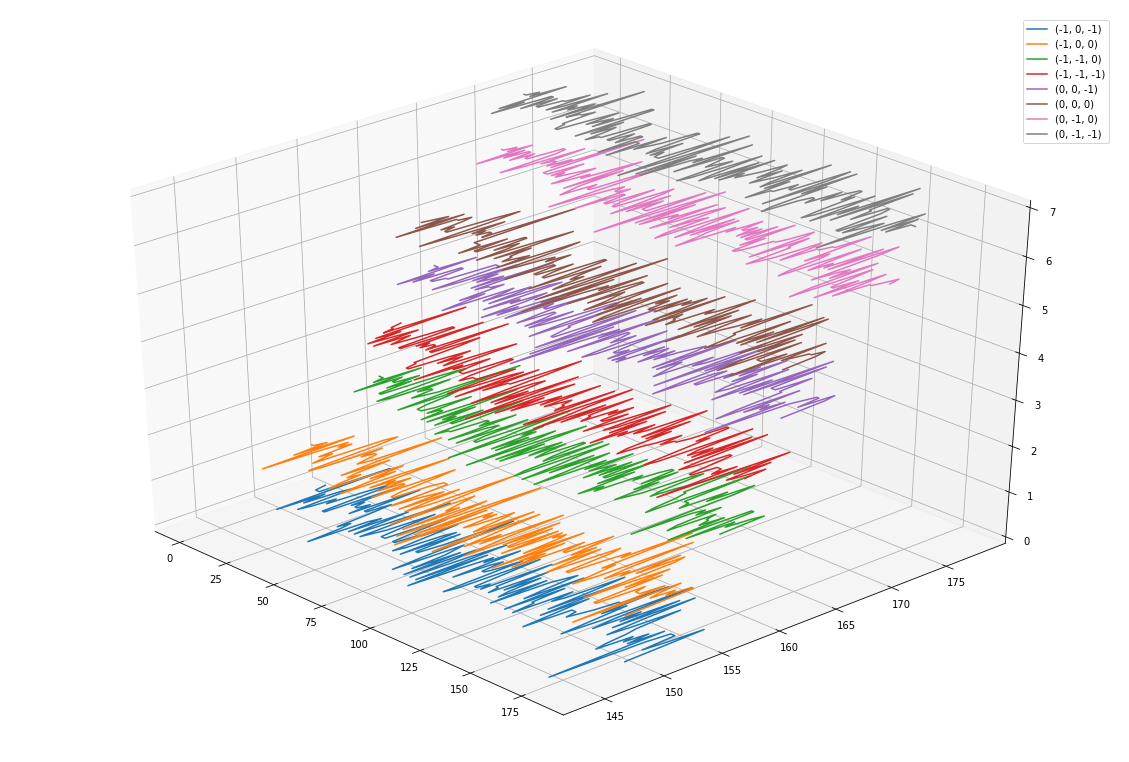
\includegraphics[width=.7\columnwidth]{./img/local_100c.png}%
	\end{center}
	\caption{Пример активности локальной окрестности вокселя в течение $\approx47$ сек}%
	\label{pic:local_100c}%
\end{figure}

\begin{figure}%
	\begin{center}
		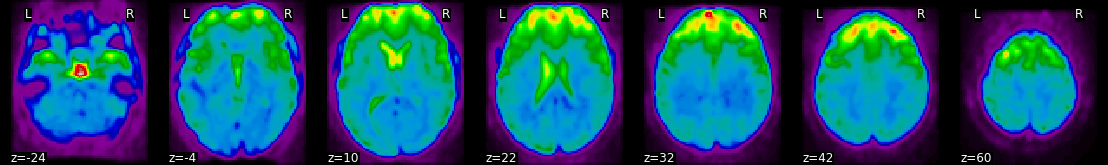
\includegraphics[width=.9\columnwidth]{./img/slices.png}%
	\end{center}
	\caption{Разрезы мозга по $z$-координате}%
	\label{pic:slices}%
\end{figure}

\section{Составление плана экспериментальных исследований разработанного алгоритма}

Что хотим

Параметры точности

Вопросы,отв на кот хотим получить

При каком числе вокселей лучше точность

\section{Исследование точности классификации при различных	способах оценки межиндивидуальных корреляций}

\section{Исследование показателей точности классификации, выявление наименее и наиболее разделимых когнитивных состояний и соответствующих зон головного мозга}

Графики, таблицы

ROC, AUC
\